\section{Durchführung}
\label{sec:Durchführung}
\subsection{Vorbereitung}
\label{sec:Vorbereitung}
Zur Vorbereitung des Versuches sollten die Fourier-Koeffizienten von drei periodischen Funktionen bestimmt werden. Bei den ausgewählten Funktionen (Sägezahn, Dreieck, Rechteck) wurde eine Vereinfachung vorgeschlagen, so dass es sich nur um gerade oder ungerade Funktionen handeln soll. 
\\
Eine gerade Funktion ist definiert als:
\begin{equation*}
\label{eqn:gerade}
f(t) = f(-t)
\end{equation*}
Bei diesem Typ verschwindet der Koeffizient $b_{n}$.
\\
Eine ungerade Funktion ist definiert als:
\begin{equation*}
\label{eqn:ungerade}
f(t) = -f(-t)
\end{equation*}
Allerdings verschwindet hier der Koeffizient $a_{n}$.
\subsubsection{Rechteckfunktion}
Die Funktion lautet:
\begin{equation*}
f(t) =
\begin{cases}
A, & -\frac{T}{2} \le t \le 0 \\
-A, & 0 \le t \le \frac{T}{2}
\end{cases}
\end{equation*}
Daraus folgt, dass $a_{n} = 0$ ist, weil $f(t)$ eine ungerade Funktion nach \ref{eqn:ungerade} ist. Nun wird der Koeffizient $b_n$ nach der Gleichung \ref{algn:Funktionen} berechnet:
\begin{align*}
b_{n} &= \frac{2}{T} \int_{\frac{-T}{2}}^{\frac{T}{2}} f(t) \text{sin}\left(n \frac{2\pi}{T} t \right) dt = \frac{2}{T} \int_{\frac{-T}{2}}^{0} A\text{sin}\left(n \frac{2\pi}{T} t \right) dt - \frac{2}{T} \int_{0}^{\frac{T}{2}} A \text{sin}\left(n \frac{2\pi}{T} t \right) dt \\
&= \frac{2}{T} \left.\left(A\frac{T}{2n\pi}\text{cos}\left(n\frac{2\pi}{T}t\right)\right)\right|_{\frac{-T}{2}}^{0} - \frac{2}{T}\left.\left(A \frac{T}{2n\pi}\text{cos}\left(n\frac{2\pi}{T}t\right)\right)\right|_{0}^{\frac{T}{2}} \\  
&= \frac{A}{n\pi}\left(\text{cos}(n\pi)-\text{cos}(0)-\text{cos}(0)+\text{cos}(n\pi)\right) \\
&= \frac{2A}{n\pi}\left(\text{cos}(n\pi)-1\right)
\end{align*}
Somit ergibt sich für $b_{n}$:
\begin{equation}
b_{n} = -\frac{4A}{n\pi}(-1)^{n},
\end{equation}
wobei $n$ ungerade ist und die Funktion ist in der Abbildung \ref{fig:rechteck} zu sehen.
\begin{figure}[htb]
	\centering
	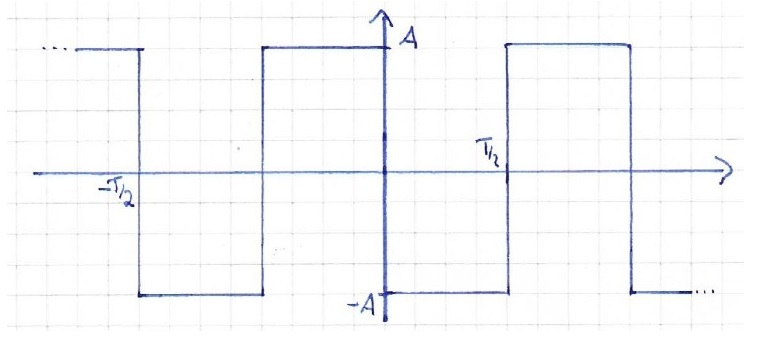
\includegraphics[width=0.7\linewidth]{../../Rechteck}
	\caption{Abbildung zur Rechtecksfunktion}
	\label{fig:rechteck}
\end{figure}
\subsubsection{Sägezahnfunktion}
Die Funktion ist in der Abbildung \ref{fig:sagezahn} zu sehen und wird gegeben als:
\begin{equation*}
f(t) = \frac{2A}{T}t
\end{equation*}
mit $a_{n} = 0 $, da $f(t)$ eine ungerade Funktion nach \ref{eqn:ungerade} ist.
\begin{figure}[htb]
	\centering
	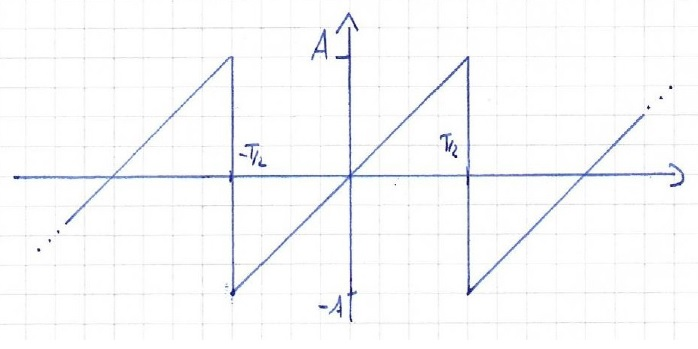
\includegraphics[width=0.7\linewidth]{../../Sagezahn}
	\caption{Abbildung zur Sägezahnfunktion}
	\label{fig:sagezahn}
\end{figure}
Nun wird hier der Koeffizient auch nach der Gleichung \ref{algn:Funktionen} berechnet. Der letzte Term verschwindet wegen des Integrals des Cosinus über eine volle Periode.
\begin{align*}
b_{n} &= \frac{2}{T} \int_{-\frac{T}{2}}^{\frac{T}{2}} \frac{2A}{T}t\sin\left(n\frac{2\pi}{T}t\right)dt = \frac{4A}{T^2}\cdot\left[-\frac{T}{2n\pi}t \left.\cos\left(n\frac{2\pi}{T}t\right)\right|_{-\frac{T}{2}}^\frac{T}{2} + {\int_{-\frac{T}{2}}^{\frac{T}{2}} \frac{T}{2n\pi}\cos\left(n\frac{2\pi}{T}t\right)dt}\right] \\
&= \frac{A}{n\pi}\text{cos}(n\pi)
\end{align*}
Somit ergibt sich:
\begin{equation}
b_{n} = A{n\pi}(-1)^{n}.
\end{equation}
\subsubsection{Dreieckfunktion}
Es erfolgt auch hier die gleiche Berechnung wie bei der Sägezahn- und Rechteckfunktion. Hier wird angenommen, dass es sich um eine gerade Funktion nach \ref{eqn:gerade} handelt.
Die Funktion lautet:
\begin{equation*}
f(t) =
\begin{cases}
+\frac{4A}{T}t+A , & -\frac{T}{2} \le t \le 0 \\
-\frac{4A}{T}+A , & 0 \le t \le \frac{T}{2}
\end{cases}
\end{equation*}
Damit verschwinden alle $b_{n}$, also $b_{n} = 0$. Die Funktion ist in der Abbildung \ref{fig:dreieck} zu sehen.
\begin{figure}[htb]
	\centering
	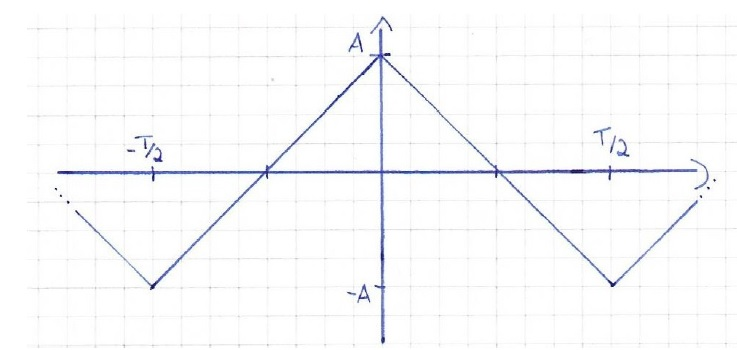
\includegraphics[width=0.7\linewidth]{../../Dreieck}
	\caption{Abbildung zu der Dreieckfunktion}
	\label{fig:dreieck}
\end{figure}
Nach der Gleichung \ref{algn:Funktionen} wird $a_{n}$ wird berechnet:
\begin{align*}
a_{n} &= \frac{2}{T} \int_{\frac{-T}{2}}^{\frac{T}{2}} f(t) \cdot \text{cos}\left(n \frac{2\pi t}{T} \right) dt \\
&= \frac{2}{T} \int_{-\frac{T}{2}}^{0} \frac{4A}{T}t  \cdot \text{cos}\left(n \frac{2\pi t}{T} \right) dt - \frac{2}{T} \int_{0}^{\frac{T}{2}} \frac{4A}{T}t \cdot \text{cos}\left(n \frac{2\pi t}{T} \right) dt + \frac{2}{T} \int_{-\frac{T}{2}}^{\frac{T}{2}} 2A\text{cos}\left(n \frac{2\pi t}{T} \right) dt 
\end{align*}
Hier verschwindet ebenfalls der letzte Termin wegen des Integrals des Cosinus über volle Periode. 
Daher ergibt sich:
\begin{equation}
a_{n} = \frac{8A}{\pi^2 n^2}
\end{equation}
wobei $n$ ungerade ist. 
\subsection{Fourier-Analyse}
Die Fourier-Analyse wird mit Hilfe der Fourier-Transformation durchgeführt. Es sollen hier die drei ausgewählten Funktionen (Sägezahn, Dreieck, Rechteck) mittels Fourier-Analyse untersucht werden. Zuerst steht in erster Reihe ein Funktionsgenerator zur Verfügung, welcher an einem Oszilloskop angeschlossen wird und ein Signal konstanter Frequenz erzeugt, welches ebenfalls über das Oszilloskop dargestellt wird. 
Das Oszilloskop besitzt im Mathemodus die Funktion, die Fourier-Transformation durchzuführen und das Frequenzspektrum der jeweiligen Spannung darzustellen. Für jede Spannung bzw. Funktion ergibt sich einen Linienspektrum wie in der Abbildung \ref{fig:linienspektrum}. Mit einem Cursor werden die Amplituden bestimmt, die Messwerte abgelesen und dann notiert. Am Ende wird dann auch die Frequenz aufgeschrieben.
\begin{figure}[htb]
	\centering
	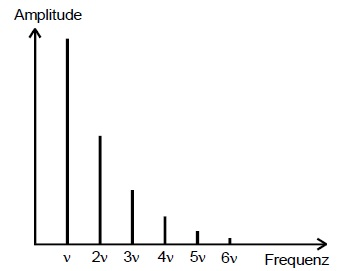
\includegraphics{../../Linienspektrum}
	\caption{Ideales Linienspektrum periodischer Funktionen,\cite[1]{anleitung351}.}
	\label{fig:linienspektrum}
\end{figure}
\subsection{Fourier-Synthese}
Bei der Fourier-Synthese werden die drei Spannungstypen aus ihren Komponenten bis $n = 9$ oder $10$ zusammengesetzt. Für diesen Teil der experimentellen Betrachtung wird ein Oberwellengenerator benutzt, der die einzelnen Schwingungen erzeugt und zusammenschaltet. Der Generator wird ebenfalls auch mit dem Voltmeter verbunden und muss in XY-Betrieb geschaltet werden um die Phasen bestimmen zu können. Zudem wird die Phasenbeziehung überprüft. An dem X-Eingang wird die 1. Grundschwingung und an dem Y-Eingang die jeweilige Oberschwingung angeschlossen. Die Phase der jeweiligen Oberschwingung wird nun so lange eingestellt, bis sich die Lissajous-Figur zu einer einzelnen Linie mit zwei Endpunkten ausgebildet hat. (vgl. Abbildung \ref{fig:lissajous} links)
\begin{figure}
	\centering
	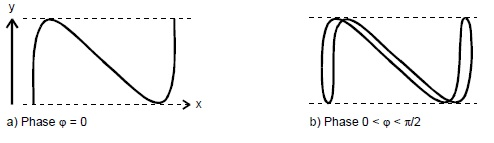
\includegraphics{../../Lissajous}
	\caption{Zwei Beispiele für Lissajous-Figuren, \cite[7]{anleitung351}.}
	\label{fig:lissajous}
\end{figure}
Die Phase beträgt jetzt nun $0$ oder $\pi$. Zwischen diesen Phasen kann nicht unterschieden werden, weshalb die einzelnen Schwingungsphasen während  der Addition der Schwingungen eventuell noch per Kippschalter verändert werden müssen. 
Im nächsten Schritt werden die Koeffizienten der drei Funktionen aus Kapitel \ref{sec:Vorbereitung} betrachtet.
Bei der Berechnung für die Rechteckspannung und für die Sägezahnspannung hat sich herausgestellt, dass die beiden Funktionen jeweils mit $\frac{1}{n}$ abfallen. Der einzige Unterschied liegt bei der Dreieckspannung wo die Funktion mit $\frac{1}{n^{2}}$ abfällt.
Die Amplituden der Oberwellen werden eingeregelt und die Ausgänge der Oberwellengenerators werden an ein AC-Millivoltmeter eingeschlossen. 

Entsprechend wird danach mit Hilfe des Ausgangs "Summenschwingung" des Generators eine Verbindung zum Oszilloskop gemacht und in "xt"- Betrieb geschaltet.
Die Phasen werden um $180$ verschoben und die einzelnen Oberwellen müssen mit Hilfe der Summationschalter aufaddiert werden.  
Bei der Rechteckspannung werden nur die ungeraden Oberwellen benutzt und die Phasen um $180$ verschoben.
Dies wird solange gemacht, bis die erwartete Schwingung angezeigt wird. 

Für die Sägezahnspannung wird der gleiche Schritt wie zuvor angewandt und die Phase neu um $180$ verschoben und solange variiert bis die entsprechende Schwingung auf dem Bildschirm angezeigt wird. Für diese Schwingung muss jedoch jede Amplitude betrachtet werden.

Bei der Dreieckspannung werden ebenfalls wie bei der Rechteckspannung auch nur ungeraden Oberwellen verwendet, die Amplituden wieder neu eingestellt und möglichst genau um $180\si{\circ}$ so verschoben.
Zudem werden die Unstetigkeitsstellen von $f(t)$ beobachtet.
Um die einzelnen Oberwellen für die drei Spannungen zu bestimmen, wird die erste eingestellte Oberwelle benötigt, die einen maximalen Wert von $U_{1} = \SI{0,678}{\volt}$ beträgt.

Bei der Rechteck- und Dreieckspannung werden nur die ungeraden Oberwellen betrachtet, und die Berechnung der einzelnen Oberwellen wird mit Hilfe der folgenden Formeln durchgeführt:
\begin{equation}
\label{eqn:Spannungungerade}
U_{2i-1} = \frac{U_{1}}{2i-1}
\end{equation}
und 
\begin{equation}
\label{eqn:SpannungDreieck}
U_{2i-1} = \frac{U_{1}}{(2i-1)^2}
\end{equation}
wobei $i = 1, 2, ...$ ist und der Nenner einfach die Teilungszahl für die ungeraden Oberwellenschwingungen entspricht. 
Bei der Sägezahnspannung wird die folgende Formel eingeführt:
\begin{equation}
\label{eqn:Spannungalle}
U_{i} = \frac{U_1}{i}
\end{equation}
wobei $i = 1, 2, ...$ ist und der Nenner die Teilungszahl für jede Oberwellenschwingung entspricht. 